\section{Hierarchically Fused Fully Convolutional Network}
\label{Sec:HF-FCN}
\subsection{Network Architecture}
 VGG16 network which is widely used in computer vision domain is regarded as the backbone network of our HF-FCN. It consists of 13 convolutional (conv) layers and 3 fully connected (fc) layers while its conv layers are divided into five groups with a pooling layer after each group. With the deepening of network, the receptive field (RF) of each activation units is increasing. Detailed receptive field and stride size of diverse layers are shown in Table \Rmnum{1}. The F1\_1 in Table \Rmnum{1} denotes the feature map generated by conv1\_1. Some modifications are made to apply to our roof extraction task including removing its fc layers and last pooling layer. The reasons of these changes are 1) The fc layer generates a fair number of parameters and takes up too much memory. 2) The existence of fc layer limits the size of input image. 3) After the last pooling layer, the resolution of the feature map is reduced to 1/32 of the input, which is too small to building extraction task.\par
\begin{table}[!h!b!p]
\centering
\caption{The receptive field and the stride size of VGG16 net}

\begin{tabular}{c||cccccc}
\hline
layer &F1\_1 &F1\_2 & Pool1 &F2\_1 &F2\_2 &Pool2 \\ \hline
RF &3&5&6&10&14&16\\ \hline
stride &1 &1 &2 &2 &2 & 4\\ \hline\hline
layer &F3\_1 &F3\_2 & F3\_3 &pool3 &F4\_1&F4\_2\\ \hline
RF &24&32&40&44&60&76\\ \hline
stride &4 &4 &4 &8 &8 &8\\ \hline\hline
layer &F4\_3&Pool4 &F5\_1 &F5\_2 &F5\_3& Pool5 \\ \hline
RF &92 &100 &132 &164 &196 &212 \\ \hline
stride &8 &16 &16 &16 &16 &32\\ \hline
\end{tabular}
\end{table}
\setlength{\parindent}{2ex}In order to leverage the information extracted from different layers, we add the fusion branches on the backbone network which fuses the prediction results obtained by different feature maps. The idea is similar to getting the response of scale function of images when looking for the SIFT feature points. After getting the responses of different scale functions, the biggest response is selected between adjacent scales of each feature point. Choosing the most suitable scale is determined by weights of fusion layers in our network. Extracting the information from different scales of receptive field as well as diverse levels of semantics is fused into a final prediction result. In addition, all of our fusion operations are learned from the network indicating that network automatically learns the connection among feature maps. The architectures of HF-FCN is shown in Fig. 1. The trimmed VGG16 Net is denoted as Level 1 in our HF-FCN. Each conv layer in Level 1 is connected to a conv layer with kernel size 1. And the outputs of these layers are upsampled and cropped into the same resolution of input image. All the up-sampling feature maps are concatenated and connected  by an 1$\times$1 conv layer, which contribute to our level 2.\par
\begin{figure*}
\centering
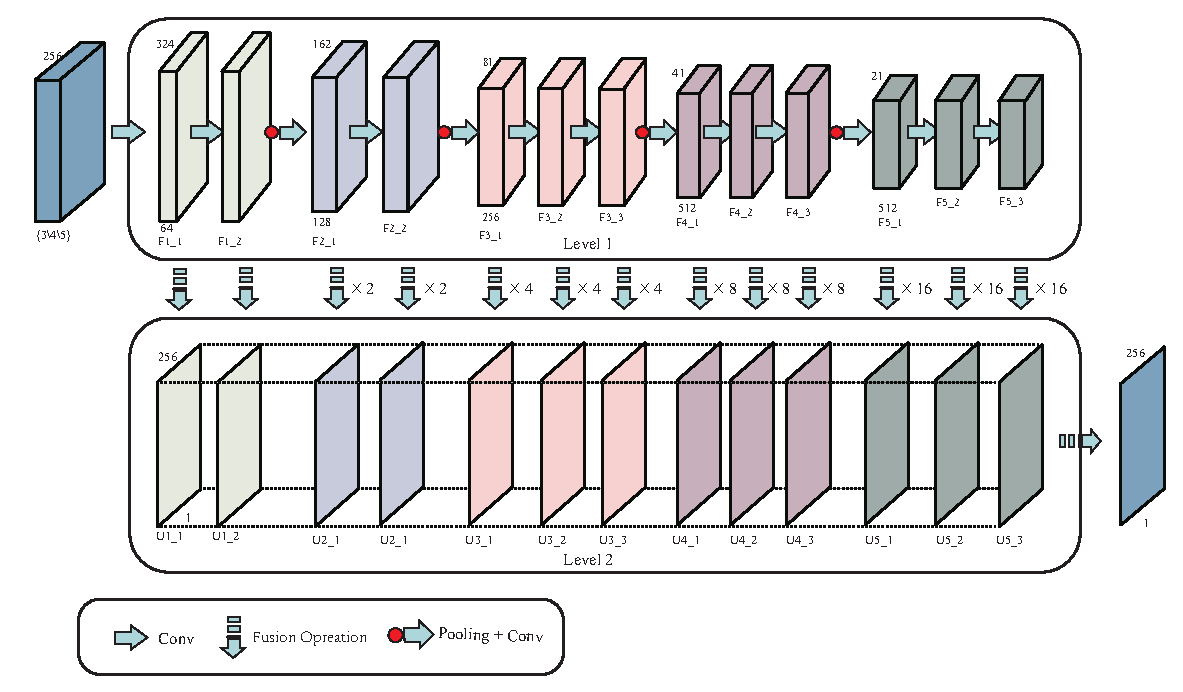
\includegraphics[width=18cm,height=9.5cm]{Figures/network_architecture.eps}
\centering
\caption{Overall architecture of HF-FCN. The action of VGG16 network is extracting features from various layers. All feature maps from various layers merge into a feature map which eliminating redundancy in the same semantics and resolution. In Level 2, 13 feature maps are up-sampled and cropped to the same size of input. Finally the cropped feature maps fuse into a prediction result. All fusion operations used in HF-FCN are 1$\times$1 convolution. The input channel could be 3, 4 or 5 for RGB, DSM, nDSM. $\times$2 means 2 times of upper sampling. U1\_1 means the upsampling of F1\_1, and so forth.  }
\label{3}
\end{figure*}
\setlength{\parindent}{2ex}In Level 1, with the growing of the receptive field, the detailed information is captured by each convolutional layer from fine-grained to coarser while the semantic information captured from low level to high level. The first fusion operation is aimed to eliminate the redundancy within the feature maps of the same size. For the task of rooftop extraction, not only the details of the appearance of the building captured by shallow layers is needed, but also the information of the line and corner extracted by middle layers and the high-level semantics which mainly comes from deep layers are needed. Hence, in Level 2, we combine hierarchical features from whole up-sampling layers into a final prediction. Figure 4 shows the upsampled feature maps from different convolutional layers. The U1\_1 in Fig. 4(b) means the upsampled feature maps from F1\_1 which are feature maps generated from conv1\_1 with small receptive field extracts low-level features like edges. In Fig. 4(c), the U1\_2 looks like an over-segmentation which groups pixels with similar color or texture into a subregion. In the U2\_1, as Fig. 4(d) shows, shape information is augmented. From the U3\_3, we can see that regions with significantly varying appearance are merged into an integrated building by considering high-level features. In U4\_3 and U5\_3, more semantic information of rooftop is got, which can distinguish the rooftop and the roads with similar color and deal with problems caused by shadow. Since all the upsampled feature maps are fused, it is expected to achieve a boost in rooftop segmentation. The final prediction result is shown in Fig. 4(h).
\begin{figure}
\centering
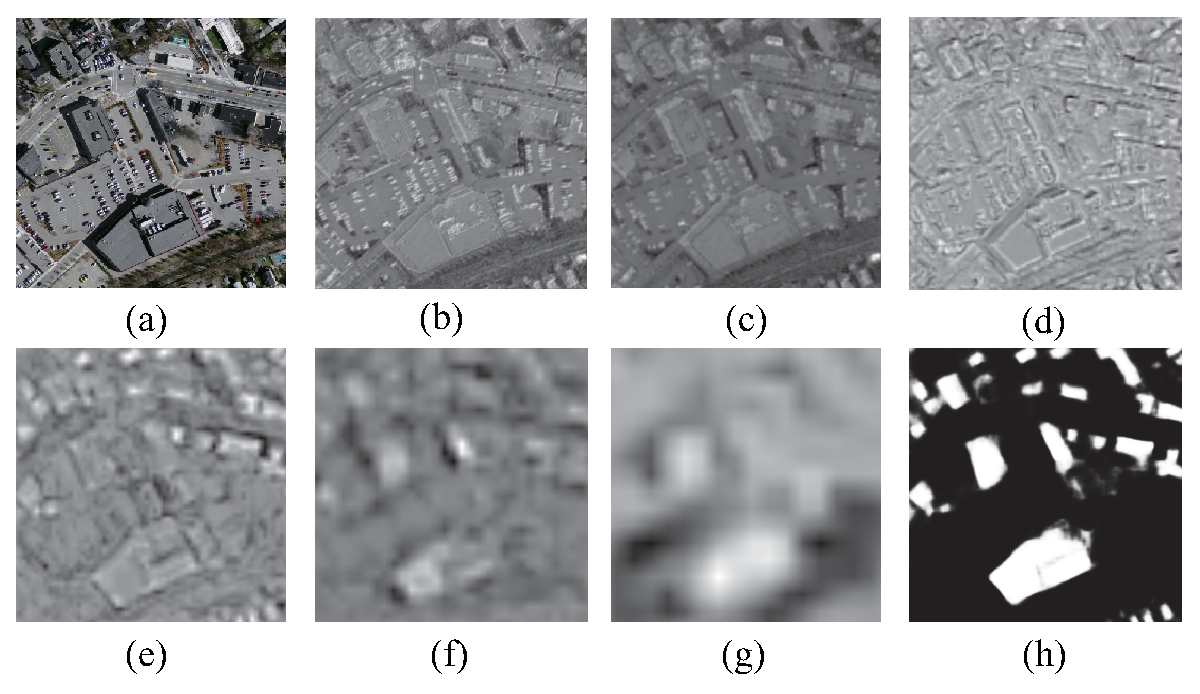
\includegraphics[width=8.7cm]{Figures/feature_maps.eps}
\caption{(a) Input aerial image. (b-g) Feature maps generated from U1\_1, U1\_2, U2\_2, U3\_3, U4\_3, U5\_3, respectively. (h) Predicted labelling map}
\label{4}
\end{figure}
\subsection{Network Training}
\setlength{\parindent}{2ex}The ground truth $M$ in our dataset is labeled by 0 or 1. Here 1,0 means that this pixel belongs to a roof or not. When a remote sensing image ${X}$ is inputted into the network, the output is a prediction probability map $P(X;W)$ of roof, where $W$ denotes all the parameters that learned by HF-FCN. Each pixel value in $P(X_{i};W)$ means the probability of this pixel belongs to rooftop. We use the sigmoid cross-entropy loss function formulated as
\begin{small}
\begin{equation}
     \label{loss}
     \ L(W)\! =\! -\frac{1}{\vert I\vert}\sum_{i=1}^{\vert I \vert}\lbrack{\tilde{m}_i \log{P(X_{i};W)}\!+\!(1\!-\!\tilde{m}_i)\log(1\!-\!P(X_{i};W)}\rbrack,
\end{equation}
\end{small}
where $\tilde{m}_i$ is label of $X_{i}$, ${\vert I\vert}$ is the number of pixels in the input image ${X}$.
